\chapter{Rooted Trees and Trees}

Rishnak found Ajur and his dog Jura walking along a row of graves. Ajur was reading the inscriptions on the tombstones. Each headstone had the names of the family (parents, wife, husband) and the dates of birth and of death. Ajur did not know so many relatives could be buried in such a small area. He then thought of how different cultures honor their departed ones. \footnote{He remembered seeing the movie Coco in 2017 about how people in Mexico remember their departed ones. He had also heard how Hindus in India go to the city of Banaras/Varanasi to perform rituals to thank and honor their deceased forefathers.} 
Ajur remembered the definition of a tree and a rooted tree. He was talking to Jura, saying that a rooted tree in graph theory/mathematics looks like a normal tree with a distinguished vertex. A rooted tree in real life has a root at the bottom whereas a rooted tree in graph theory is drawn with a root at the top. Both of them convey the same information.

``Here are two drawings of the same information." Ajur further explained that each vertex in a rooted tree has just one parent vertex (except the root vertex, which has no parent). A rooted tree can also be thought of as a graph with a collection of vertices and edges. There are some restrictions. But that will become clearer, as the story proceeds.


\begin{figure}
\begin{center}
\includegraphics[width=\textwidth]{tree1.JPG}
\caption{A Tree drawn with a root at the bottom}\label{rg1}
\end{center}
\end{figure}

\begin{figure}
\begin{center}
\includegraphics[width=\textwidth]{tree2.JPG}
\caption{Same Tree drawn with a root at the top}\label{rg2}
\end{center}
\end{figure}

Rishnak caught up with Ajur and Jura as he had been following them quietly. Rishnak asked Ajur: ``How many edges does a rooted tree with 7 vertices have?" Ajur reasoned that since each vertex other than the root has exactly one parent vertex and there are no other edges, then number of edges will be 6. Rishnak then asked how many edges a rooted tree with 1000 vertices has. Ajur shot back with his answer 999. Impressed, but not unduly, Rishnak asked how many edges there are in a rooted tree with $n$ vertices. Nonchalantly, Ajur replied it is $n-1$ by the same argument (each of the $n-1$ vertices have just one edge connected to its parent).  

For each vertex other than a root vertex, there is a parent vertex and zero or more child vertices.  The descendants of a vertex are all its children, grandchildren, great grandchildren vertices, etc. Analogously, for each vertex the ancestors of that vertex are its parent, grandparent, great grandparent vertices, etc. 
A vertex with no child vertices is known as a leaf vertex. Rishnak asked Ajur ``What is the largest number of leaf vertices a tree with 6 vertices can have?" Ajur immediately responded that the number is 5, and he drew a rooted tree as in Figure \ref{t1}.

\begin{figure}
\begin{center}
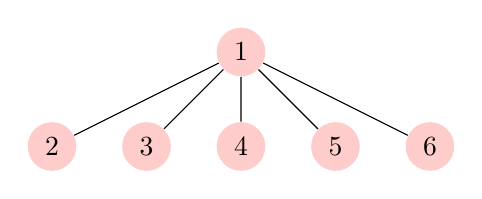
\begin{tikzpicture}
  [scale=.6,auto=left,every node/.style={circle,fill=red!20}]
  \node (n6) at (5,5) {1};
  \node (n4) at (1,3)  {2};
  \node (n5) at (3,3)  {3};
  \node (n1) at (5,3) {4};
  \node (n2) at (7,3)  {5};
  \node (n3) at (9,3)  {6};

  \foreach \from/\to in {n6/n1,n6/n2,n6/n3,n6/n4,n6/n5}
    \draw (\from) -- (\to);

\end{tikzpicture}
\caption{A Tree with 6 vertices and 5 leaf vertices. The vertex labeled 1 is the root vertex}\label{t1}
\end{center}
\end{figure}

Rishnak asked, ``What is the smallest number of leaf vertices a tree with 6 vertices can have?" Ajur knew this answer too. So he drew a rooted tree as in Figure~\ref{t2}.

\begin{figure}
\begin{center}
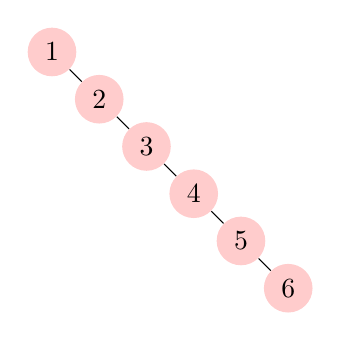
\begin{tikzpicture}
  [scale=.6,auto=left,every node/.style={circle,fill=red!20}]
  \node (n6) at (3,7) {1};
  \node (n4) at (4,6)  {2};
  \node (n5) at (5,5)  {3};
  \node (n1) at (6,4) {4};
  \node (n2) at (7,3)  {5};
  \node (n3) at (8,2)  {6};

  \foreach \from/\to in {n6/n4,n4/n5,n5/n1,n1/n2,n2/n3}
    \draw (\from) -- (\to);

\end{tikzpicture}

\caption{A Tree with 6 vertices and one leaf vertex labeled 6. The vertex labeled 1 is the root vertex.}\label{t2}
\end{center}
\end{figure}

Rishnak said, ``We get a lot of lightning and thunderstorms here, especially during summer months. Lightning affects tall objects, especially objects that conduct electricity in an open area.\footnote{Benjamin Franklin had demonstrated the electrical nature of lightning.} Lightning conductors are usually at the top of the buildings and have less resistance than the building and hence lightning passes through the conductor." Rishnak drew a rooted tree with 3 vertices as shown in Figure~\ref{t3}.

\begin{figure}
\begin{center}

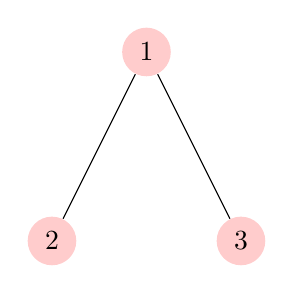
\begin{tikzpicture}
  [scale=.6,auto=left,every node/.style={circle,fill=red!20}]
  \node (n1) at (3,7) {1};
  \node (n2) at (1,3)  {2};
  \node (n3) at (5,3)  {3};


  \foreach \from/\to in {n1/n2,n1/n3}
    \draw (\from) -- (\to);

\end{tikzpicture}

\caption{A resistance  Tree with 3 vertices and two leaf vertices at the ground. }\label{t3}
\end{center}
\end{figure}


Rishnak said that the each edge has a resistance of 1 ohm, and vertices labeled 2 and 3 are grounded. What is the effective resistance of the resistance tree in Figure~\ref{t3}? Ajur remembered his physics and he realized two resistances are in parallel. So he immediately replied that the effective resistance is $\frac{1}{2}$ ohms. (Intuitively, there are two paths the current can take and hence the resistance splits evenly between the two paths).

Rishnak asked the same question, effective resistance, for the following rooted tree shown in Figure \ref{t4}.
\begin{figure}
\begin{center}

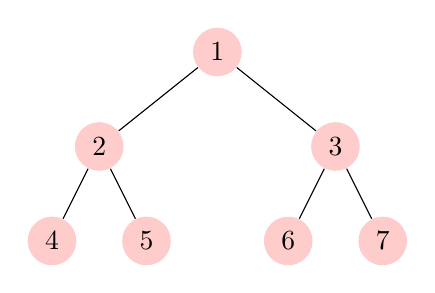
\begin{tikzpicture}
  [scale=.6,auto=left,every node/.style={circle,fill=red!20}]
  \node (n1) at (5.5,7) {1};
  \node (n2) at (3,5)  {2};
  \node (n3) at (8,5)  {3};
  \node (n4) at (2,3) {4};
  \node (n5) at (4,3)  {5};
  \node (n6) at (7,3)  {6};
  \node (n7) at (9,3)  {7};

  \foreach \from/\to in {n1/n2,n1/n3,n2/n4,n2/n5,n3/n6,n3/n7}
    \draw (\from) -- (\to);

\end{tikzpicture}

\caption{A resistance  Tree with 7 vertices and four leaf vertices at the ground. }\label{t4}
\end{center}
\end{figure}

Ajur said that he had computed the effective resistances for trees rooted at vertex labeled 2 and 3 to be $\frac{1}{2}$. There are two parallel paths with equal resistance of $1+\frac{1}{2}$ (There is a series connection from root vertex 1 and vertices labeled 2 and 3 respectively). Hence the effective resistance is $\frac{3}{4}$ ohms. Ajur further said that there is a pattern here. For the resistance tree with 15 vertices (adding one more level or increasing the height), the effective resistance will be $\frac{7}{8}$. Rishnak then asked what happens if the tree is of infinite height! (A really tall lightning conductor.) Ajur was perplexed - But, then, he reasoned that this could be formulated as a recurrence relation. Let R be the effective resistance of this infinite tree. The root has two children, each of which will have a resistance of R ohms. The root vertex is connected to the child vertex with a resistance of 1 ohm. Hence he wrote an equation $$R= \frac{R+1}{2}$$ Simplifying this, he got the resistance of 1 ohm. A tree of infinite height with its very low resistance is like a really tall and effective lightning conductor.\footnote{Because of a large number of joints, this solution may not be a practical one!} Rishnak responded that there is another way of getting the same result. From an earlier example, you can generalize the resistance to be $\frac{2^h-1}{2^h}$ , $h$ being height (longest among path lengths from the root vertex to all leaf vertices) of the rooted tree. This can be further simplified to be $1-\frac{1}{2^h}$. As $h$ goes to infinity the term $\frac{1}{2^h}$ goes to 0 and hence the resistance is 1. Ajur learned an important lesson that there are multiple ways of getting a solution and each one may provide a new insight. Ajur asked Rishnak: ``Can you construct an infinite height tree (with edge resistances being 1 ohm) so that the effective resistance is $\frac{1}{2}$, $\frac{1}{3}$, $\frac{1}{4}$ or more generally any fraction $\leq$~1?" Rishnak replied to Ajur that he was the one who could ask questions and not Ajur.\footnote{Of course, Rishnak knew the answer and suggests others to think of every vertex having more than 2 child vertices!}

A tree is like a rooted tree but with no root vertex. A tree can be drawn in any manner. The degree of a vertex is the number of edges incident on that vertex. The leaf (pendant) vertex has a degree of 1. So in Figure~\ref{t2} both vertices labeled 1 and 6 are leaf/pendant vertices and all other vertices have degree 2. 

Rishnak told Ajur that one important property of a tree is that there are no cycles in it. Ajur could easily understand it from a genealogy perspective - a person cannot be an ancestor as well as a descendant of himself/herself.  Ajur added that there is only one path between any two vertices in a tree (Of course, Ajur assumed that the edges are undirected - which Rishnak knew). Rishnak asked ``how did you infer that there is a unique path between two vertices in a tree?" Ajur promptly replied that if there are two paths between any two vertices, there will be a cycle (which cannot exist in a tree). Since there is a unique path between two vertices, one can compute the distance between two vertices as the number of edges in that path. Ajur provided clarifications with examples.  As an example in Figure~\ref{t1}, the distance between the vertex labeled 1 and any other vertex is 1. The distance between the vertex labeled 2 and the vertex labeled 6 is 2. In Figure~\ref{t2}, the distance between the vertex labeled 1 and the vertex labeled 6 is 5 and the distance between the vertex labeled 2 and the vertex labeled 4 is 2.
%(Dad: you could also add the fact that every finite tree has a center of mass! it's in this vein, and not especially well known (Boris hadn't realized it!))

\textbf{Question for the second day:} Construct an infinite tree with resistance of $\frac{3}{5}$.

\textbf{Answer:} Ajur said a way to think about this is to consider an infinite tree in which vertex has 6 children and each edge is of resistance 3 ohms (We can add a series of three 1 ohm edges to get 3 ohms).
With this we will get a recurrence equation $R=\frac{R+3}{6}$ - that is, each child vertex will have a resistance of R ohms (by symmetry as they look like the original tree). Simplifying this, we will get a $\frac{5R}{6}=\frac{3}{6}$ which simplifies to a resistance, R, of $\frac{3}{5}$ ohms.

Rishnak was very pleased. They called it a day.